\documentclass[
    aps,
    prl,
    reprint,
    10pt,
    amsmath,
    amssymb,
    a4paper,
    longbibliography
]{revtex4-2}

\usepackage{
    graphicx,
    dcolumn,
    amsmath,
    amsfonts,
    amsthm,
    datetime,
}
\usepackage[separate-uncertainty=true]{siunitx}
\usepackage[margin=2cm]{geometry}
\graphicspath{{figures/}}
\bibliographystyle{apsrev}

\begin{document}

\title{Measurement of the speed of light}
\author{T.D. Schanzer (z5310829)}
\affiliation{
    School of Physics, %
    University of New South Wales, %
    Sydney NSW 2052, Australia
}
\collaboration{Cohort A, Monday 9 a.m.~---~12 p.m.}
\noaffiliation
\collaboration{XXXX words}
\noaffiliation
\date{\currenttime~\today}

\begin{abstract}
    This report presents measurements of the speed of light and refractive
    index in air, acrylic glass and water using a simple teaching apparatus.
    The quality of the method and its limitations are assessed.
\end{abstract}

\maketitle

\section{Introduction}

Measurements of the speed of light have a long history, with discussion of
whether or not it was finite traced back to the ancient Greeks.
R{\o}mer (1676) is usually credited with making the first accurate
measurements for his observation of variations in Io's eclipse durations
behind Jupiter as the Earth approached and receded in its annual orbit
\cite{spence_history}.

More sophisticated experiments later increased the precision with which
the speed of light was known, to the point that it could be given an
exact value in SI units in a 1983
resolution of the seventeenth General Conference on Weights and Measures.
Presently, the metre ``is defined by taking
the fixed numerical value of the speed of light in vacuum, $c$, to be
299 792 458 when expressed in the unit \si{\meter \per\second}''
\cite{sibrochure}.

Refractometry, the measurement of refractive indices, has many
applications in modern research, industry and medicine. These include
concentration measurements of dissolved material in liquids (e.g., sugar
in drinks), characterisation of glasses and plastics (e.g., for use in
lenses) and analysis of biofluids (e.g., blood and urine)
\cite{meeten_measurement}.

\textbf{Modern Methods} \newline
Modern methods for measuring the refractive indices of other materials
are numerous. Meeten (2014) \cite{meeten_measurement} describes several,
including:

\emph{Interferometry.} An interferometer separates a laser into two beams,
one of which travels through air and the other through the medium of
interest, before recombining them to produce a pattern of interference
fringes from which the phase difference and refractive index can be
determined.

\emph{Deviation.} A beam of light is passed at an angle through a flat
sheet of the material with known thickness. The beam that emerges on the
other side of the sheet is parallel to the incident beam but offset
laterally due to refraction. The magnitude of the deviation can be
related to the refractive index, thickness and angle of incidence using
Snell's Law.

\emph{Critical angle (Abbe method).} The incidence angle at which light,
passing from the medium of interest into a medium of known lower
refractive index, is refracted at $\ang{90}$ is found by measuring the
reflectance or transmittance at the interface as a function of
incidence angle. The refractive index is easily calculated using Snell's
Law. This method is commonly used in commercial refractometers.

\textbf{The Refractive Index of Air} \newline
Many experiments, including the one detailed here, are not conducted in
vacuum and must therefore account for the refractive index of air, which
is known to depend on wavelength, temperature, pressure and relative
humidity. A commonly-used empirical formula was developed by Edl{\'e}n
in 1966 and later revised by Birch and Downs in 1994 to better match
experimental results \cite{birchdowns}. The revised formula calculates
the refractive index n three steps: the first defines an intermediate
quantity
\begin{multline}
    n_\mathrm{s} = 1 + 10^{-8} \\
    \times \left(
        8342.54
        + 2406147 \left[
            130 - \left(\sigma / \si{\per\micro\meter}\right)^2
        \right]^{-1} \right. \\
        \left. + 15998 \left [
            38.9 - \left(\sigma / \si{\per\micro\meter}\right)^2
        \right]^{-1}
    \right)
    \label{edlen1}
\end{multline}
to account for dispersion (wavelength dependence);
$\sigma = 1/\lambda$ is the
wavenumber of the light in vacuum. The second step defines another
intermediate quantity
\begin{multline}
    n_\mathrm{tp} = 1 + \frac{(p / \si{\pascal})n_\mathrm{s}}{96095.43} \\
    \times \frac{
        \left[
            1 + 10^{-8} (0.601 - 0.00972 T / \si{\celsius})p / \si{\pascal}
        \right]
    }{
        1 + 0.003661 T / \si{\celsius}
    }
    \label{edlen2}
\end{multline}
accounting for the air pressure $p$ and temperature $T$. The final value
is
\begin{multline}
    n_\mathrm{a} = n_\mathrm{tp} - (f/\si{\pascal}) \\
    \times \left [
            3.7345 - 0.0401 \left(\sigma / \si{\per\micro\meter}\right)^2
    \right] \times 10^{-10},
    \label{edlen3}
\end{multline}
where $f$ is the partial pressure of water vapour.

The conditions measured in this experiment (using an inexpensive electronic
weather station) were
$T = \SI{20.4 \pm 1}{\celsius}$,
$p = \SI{1028 \pm 2}{\hecto\pascal}$ and
relative humidity $\mathrm{RH} = \SI{47 \pm 10}{\percent}$
with an estimated wavelength $\lambda = \SI{630}{\nano\meter}$, which when
substituted into (\ref{edlen1}), (\ref{edlen2}) and (\ref{edlen3})
yield
\begin{equation}
    n_\mathrm{a} = 1.000275.
\end{equation}
By comparison to experimental results, Birch and Downs estimated the
$1\sigma$ uncertainty of the formula to be $\SI{e-8}{}$ \cite{birchdowns},
but given the uncertainty in $T$, $p$, $\mathrm{RH}$ and $\lambda$ this is
more likely to be on the order of $\SI{e-6}{}$ \cite{emtoolbox}, which
is nonetheless negligible in comparison to the uncertainties in the
results presented in this report.


\section{Aim}

This experiment seeks to determine the speed of light and refractive
index in air, acrylic glass and water.


\section{Methods}

The experiment used a combined laser source and detector unit (PHYWE
11226-00), containing a red laser source whose intensity was modulated
at $\SI{50}{\mega\hertz}$. The laser passed along an optical bench to
a reflector mounted at a variable position $x$, was reflected back to the unit
and directed onto a photodiode by a retro-reflector, as shown in Figure
\ref{setup}. The modulation of the laser intensity created pulses in both
the source signal and the intensity measured by the photodiode, allowing
the time difference between them to be measured on a digital
oscilloscope (Tektronix TBS-1072B) connected to the source/detector unit.
An illustration of this time measurement is shown in the top panel of
Figure \ref{setup}.

\begin{figure}[ht]
    \centering
    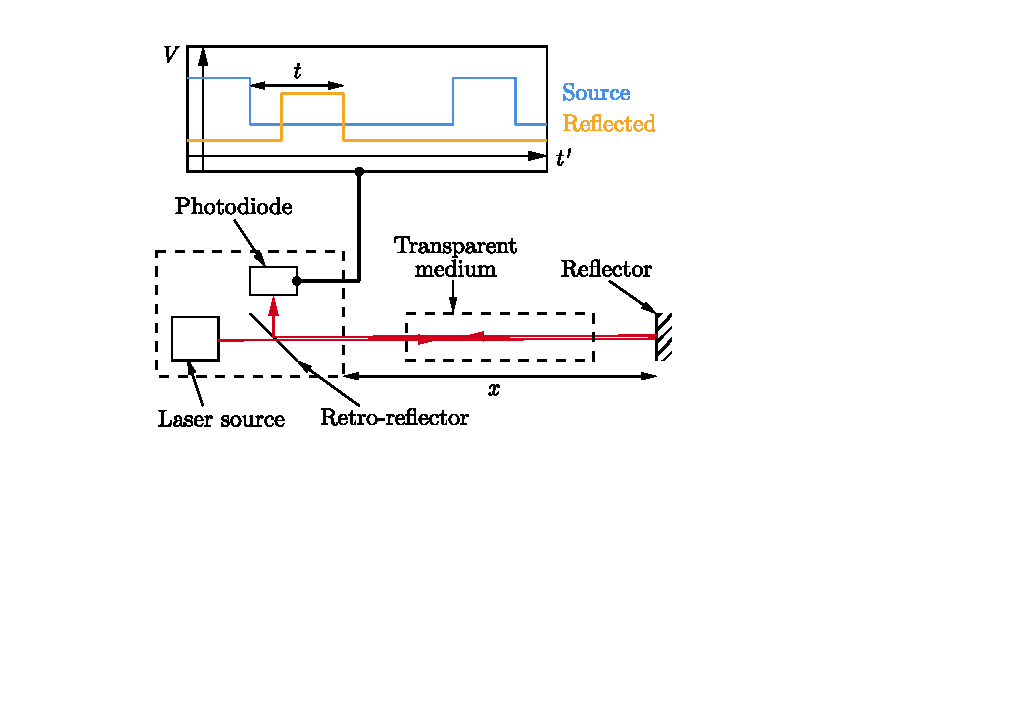
\includegraphics[width=\linewidth]{setup_updated}
    \caption{Experimental setup, showing model oscilloscope trace (top).}
    \label{setup}
\end{figure}

The speed of light in air, $c_\mathrm{a}$, was calculated by measuring
the time difference $t$ between the emitted and reflected beams as a
function of the reflector's position $x$ relative to a reference
point and performing a linear regression using the simple relation
\begin{equation}
    2x = c_\mathrm{a} t.
    \label{air_formula}
\end{equation}

Two different approaches were compared for measuring the speed of
light in transparent media, namely acrylic and water.

\emph{$\Delta x$ method.} A cylinder of the transparent medium was placed
in the path of the laser as shown in Figure \ref{setup} and the
source/detector unit calibrated to show a zero time difference between
the emitted and reflected beams. The cylinder was then removed,
shortening the time taken by the light, and the reflector moved horizontally
until the oscilloscope again showed a zero time difference, indicating
that the initial and final optical path lengths were equal. Mathematically,
\[
    2 n_\mathrm{a} x' = 2 n_\mathrm{a} (x - l) + 2 n_\mathrm{m} l,
\]
where $x$ and $x'$ are the initial and final reflector positions, $l$ is
the length of the cylinder and $n_\mathrm{m}$ is the refractive index of the
medium. Consequently,
\[
    n_\mathrm{m} = \frac{n_\mathrm{a} (x' - x + l)}{l}.
\]

\emph{$\Delta t$ method.} As before, the medium was placed in the optical
path and the source/detector unit calibrated to show a zero time
difference. The medium was removed and the resulting reduction in
travel time $\Delta t$ measured. Knowing that
\[
    \Delta t = 2 l \left(
        \frac{1}{c_\mathrm{m}} - \frac{1}{c_\mathrm{a}}
    \right),
\]
where $c_\mathrm{m}$ and $c_\mathrm{a}$ are the speeds of light in the
medium and air respectively, it follows that
\[
    n_\mathrm{m} = \frac{c}{c_\mathrm{m}}
    = \frac{c \Delta t}{2 l} + \frac{c}{c_\mathrm{a}}.
\]

\section{Results}

The linear regression of distance travelled against time according
to (\ref{air_formula}), shown in Figure \ref{air_plot}, gives a speed of
light in air of
\[
    c_\mathrm{a} = \SI{2.941 \pm 0.016e8}{\meter \per\second},
\]
with the uncertainty ($0.53\%$) accounting for uncertainties in $2x$
of $\SI{5}{\milli\meter}$ and in $t$ of $\SI{80}{\pico\second}$.
This value deviates from the accepted speed of light in air by
$3.6 \sigma$ or $1.9\%$, for reasons proposed in the Discussion.

\begin{figure}[ht]
    \centering
    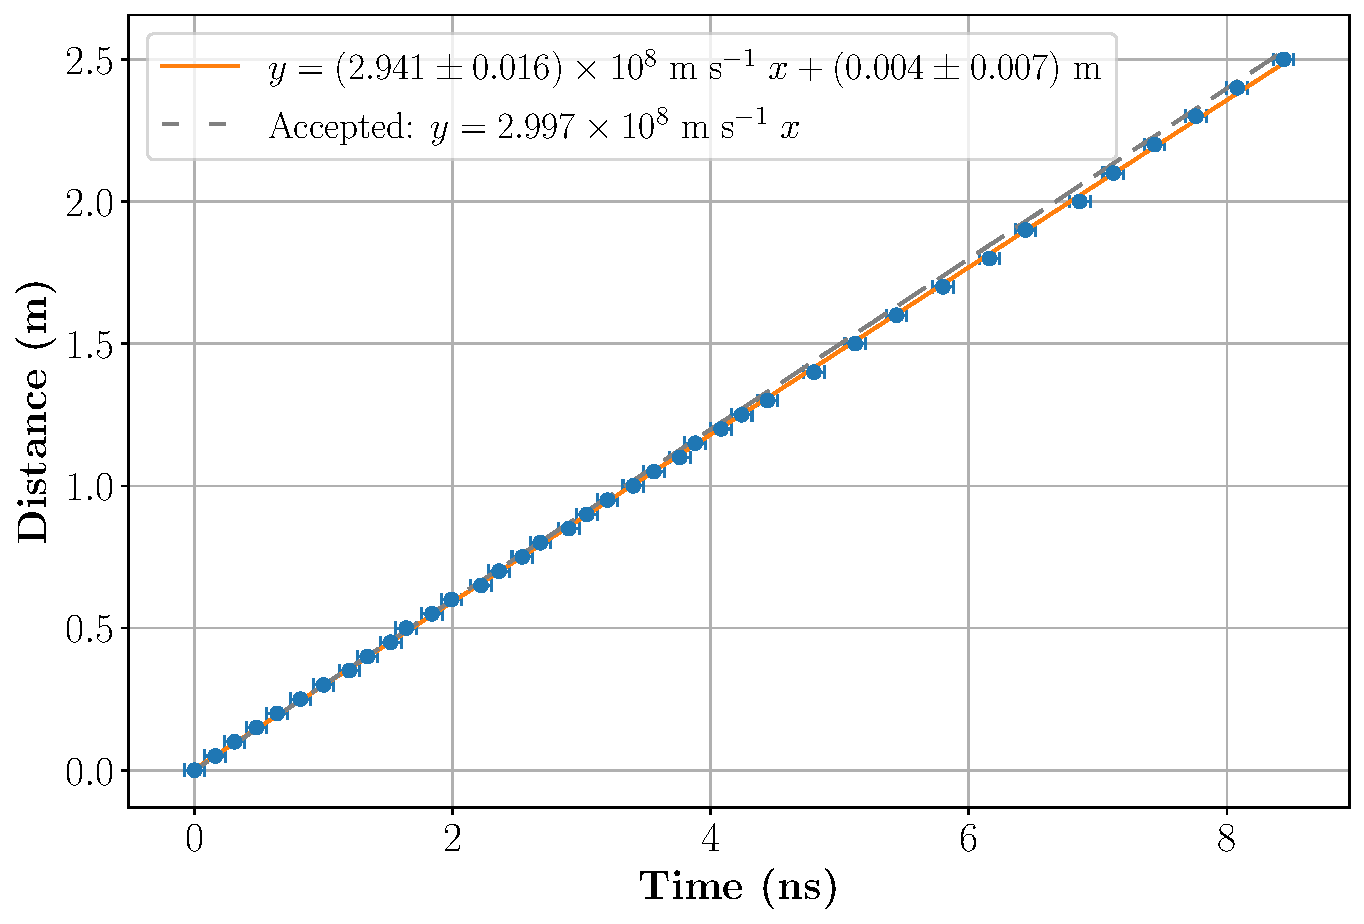
\includegraphics[width=\linewidth]{air}
    \caption{Plot of $2x$ vs. $t$ in air, with gradient $c_\mathrm{a}$.}
    \label{air_plot}
\end{figure}

Figure \ref{acrylic_plot} displays the results of the $\Delta x$
(conducted on two occasions) and $\Delta t$ methods in acrylic.
The results of an alternative method of analysis for the $\Delta x$
method are included for comparison, using the fact that
\[
    x' = x + l \left( \frac{n_\mathrm{m}}{n_\mathrm{a}} - 1 \right)
\]
to obtain $n_\mathrm{m}$ from the y-intercept of the linear regression line of
$x'$ and $x$. None of the methods agree with the accepted range of refractive
indices, $1.48 - 1.52$, provided by the manufacturer
\cite{phywebrochure}.

\begin{figure}[ht]
    \centering
    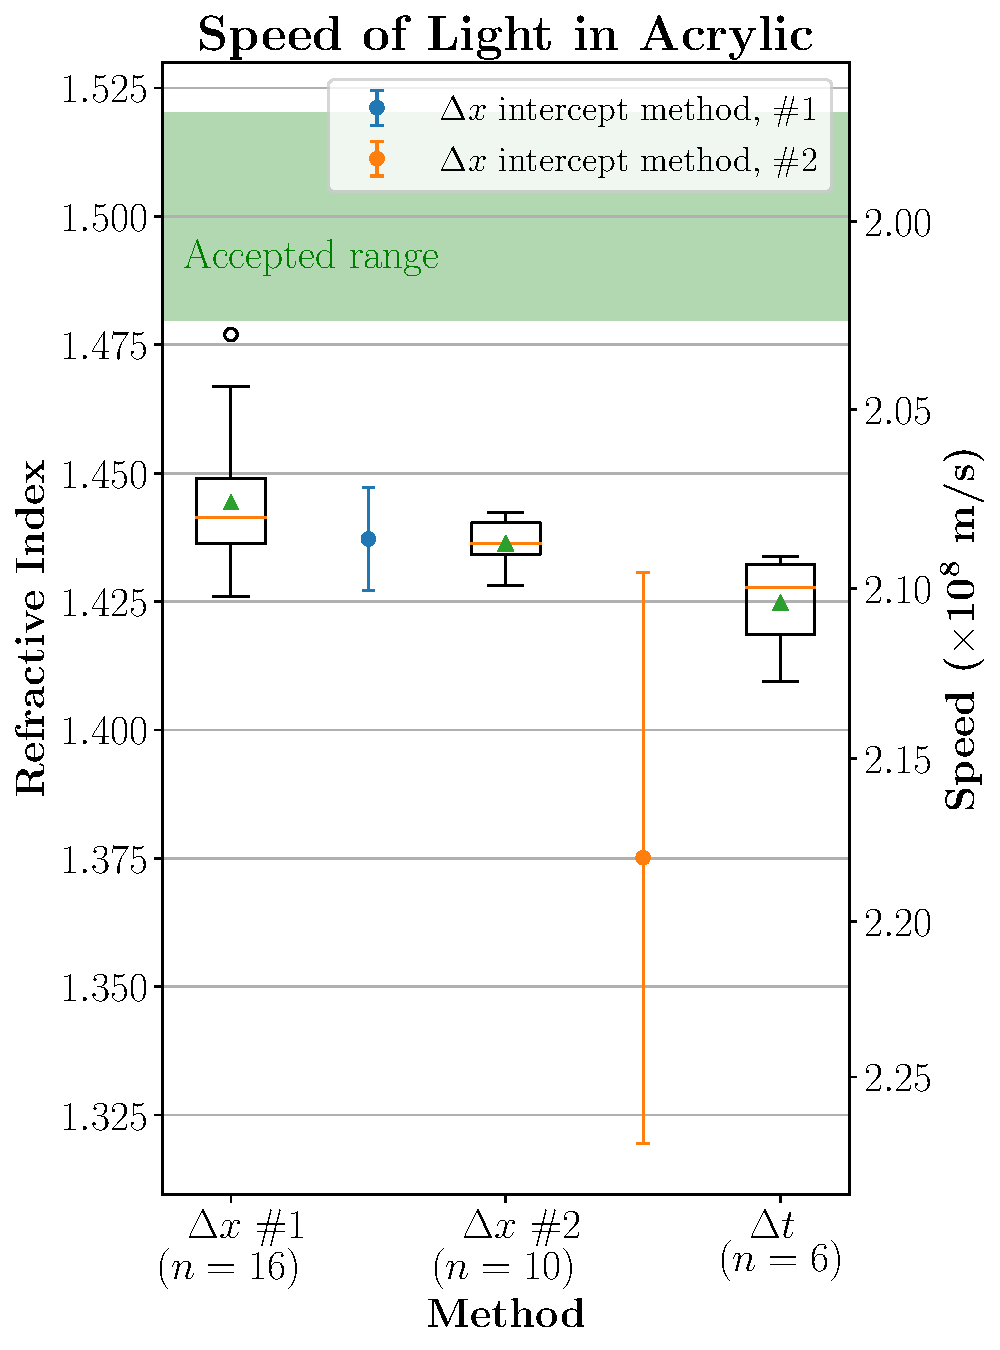
\includegraphics[width=0.7\linewidth]{acrylic}
    \caption{Measured values of the speed of light in acrylic using
        the $\Delta x$ and $\Delta t$ methods. Green triangles are
        the mean values.}
    \label{acrylic_plot}
\end{figure}

The same methods were applied for water, with the results shown in Figure
\ref{water_plot}. Only the intercept method for the second $\Delta x$
measurement seems to be in agreement with the accepted refractive index
of $1.33$, but has a much larger uncertainty and deviates significantly
from the other results.

\begin{figure}[ht]
    \centering
    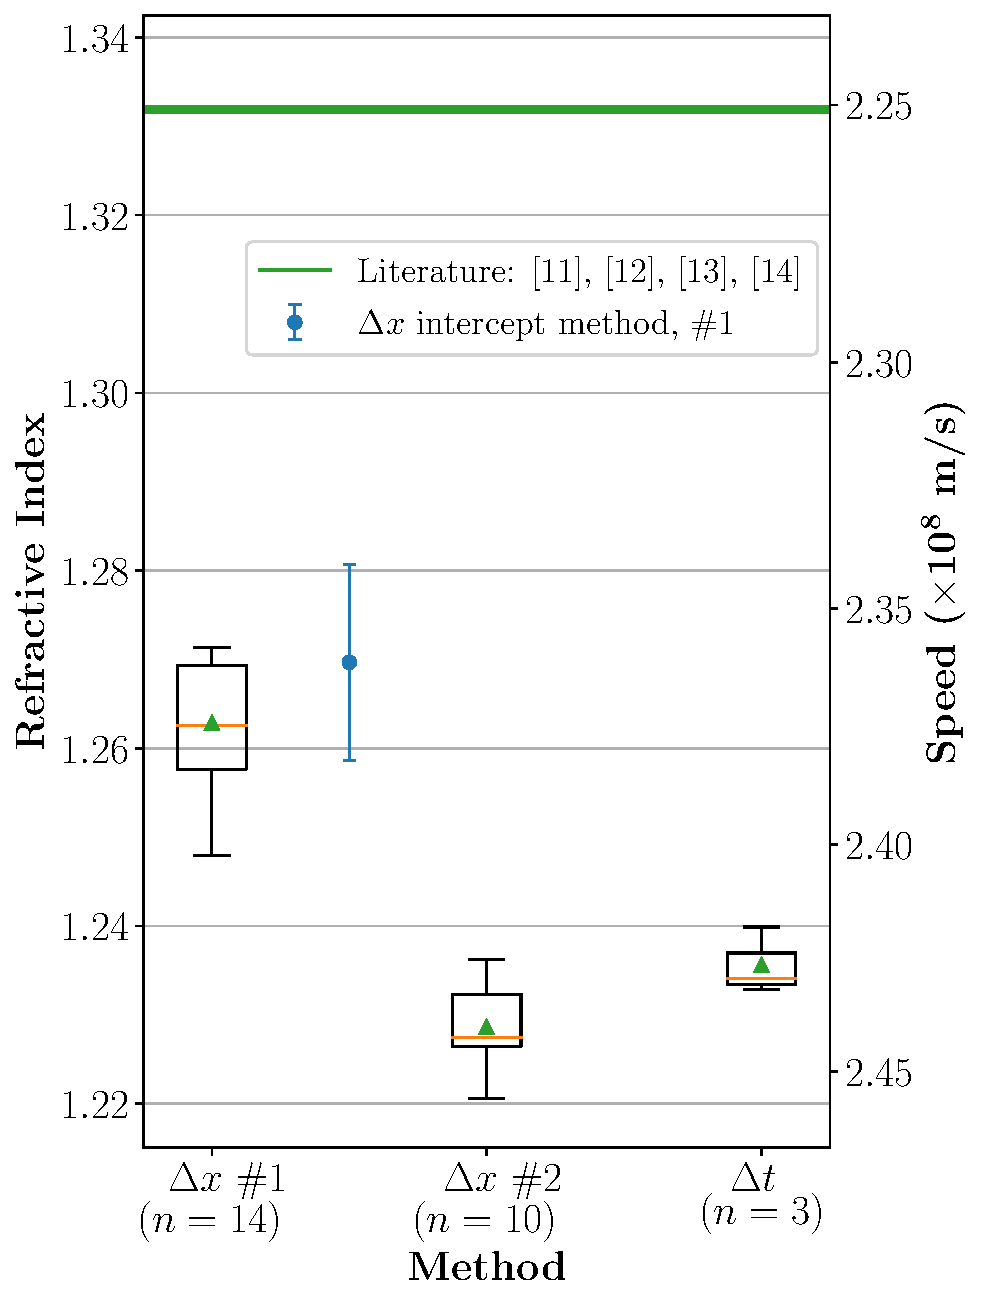
\includegraphics[width=0.7\linewidth]{water}
    \caption{Measured values of the speed of light in water using
        the $\Delta x$ and $\Delta t$ methods. Green triangles are
        the mean values.}
    \label{water_plot}
\end{figure}

\begin{table}[ht]
    \begin{tabular}{|c|c|c|}
        \hline
        \textbf{Material}
        & $n$
        & $c$ ($\times \SI{e8}{\meter \per\second}$) \\
        \hline
        \hline
        Air & $1.019 \pm 0.005$ & $2.941 \pm 0.016$ \\
        \hline
        Acrylic ($\Delta x$ \#2) & $1.436 \pm 0.004$ & $2.087 \pm 0.006$ \\
        \hline
        Acrylic ($\Delta t$) & $1.425 \pm 0.009$ & $2.104 \pm 0.014$ \\
        \hline
        Water ($\Delta x$ \#2) & $1.229 \pm 0.004$ & $2.440 \pm 0.009$ \\
        \hline
        Water ($\Delta t$) & $1.236 \pm 0.003$ & $2.426 \pm 0.006$ \\
        \hline
    \end{tabular}
    \caption{Summary of results.}
    \label{results_table}
\end{table}


\section{Discussion}

It is proposed that the disagreement between the measured and accepted
values arose from the following factors that were very difficult to
control:

\emph{Misalignment.} There was a significant amount of play in the
sliding mechanism of the reflector, making it necessary to support it
with strips of paper to render the reflected beam horizontal. Furthermore,
it was very difficult to ensure that the acrylic and water cylinders
were exactly parallel to the beam with the equipment available. Both
factors made it difficult to obtain an accurate measurement of the path
length.

\emph{Imperfect cylinder shape.} It is likely that the ends of the
acrylic and water cylinders were not exactly parallel to each other,
causing refraction and increasing the actual path length even with
good alignment. The fact that the observed time difference between
the emitted and reflected beams varied as the cylinders were rotated
supports this hypothesis.


\section{Conclusion}

The speed of light and refractive index in air, acrylic glass and water
were measured, but none were in agreement with accepted values, likely
due to inevitable misalignment of the very simple apparatus and
imperfection in the manufacturing of the acrylic and water cylinders.


\section{Acknowledgements}

The author wishes to acknowledge his fellow students Marnie Separovich
and Winnie Tang, and Prof. Chris Tinney for their valuable discussions
and suggestions.


\bibliography{references}

\end{document}
